%%%%%%%%%%%%%%%%%%%%%%%%%%%%%%%%%%%%%%%%%%%%%%%%%%%%%%%%%%%%%%%%%%%%%%%%
% Regime-Switching Ensemble (RSE) for Deep Hedging
% Top Conference-Level Research Paper
% Author: Pratham Kailasiya, IIT Roorkee
%%%%%%%%%%%%%%%%%%%%%%%%%%%%%%%%%%%%%%%%%%%%%%%%%%%%%%%%%%%%%%%%%%%%%%%%
\documentclass[11pt]{article}

\usepackage[utf8]{inputenc}
\usepackage[T1]{fontenc}
\usepackage{amsmath,amssymb,amsthm}
\usepackage{mathtools}
\usepackage{graphicx}
\usepackage{booktabs}
\usepackage{multirow}
\usepackage{tabularx}
\usepackage{threeparttable}
\usepackage{siunitx}
\usepackage{algorithm}
\usepackage{algorithmic}
\usepackage{hyperref}
\usepackage{cleveref}
\usepackage{natbib}
\usepackage{tikz}
\usetikzlibrary{shapes.geometric,arrows.meta,positioning,fit,calc}
\usepackage{pgfplots}
\pgfplotsset{compat=1.17}
\usepackage{subcaption}
\usepackage{xcolor}
\usepackage{tcolorbox}
\usepackage{enumitem}
\usepackage[margin=1in]{geometry}
\usepackage{microtype}
\usepackage{nicefrac}
\usepackage{longtable}
\usepackage{float}

\newtheorem{theorem}{Theorem}[section]
\newtheorem{lemma}[theorem]{Lemma}
\newtheorem{proposition}[theorem]{Proposition}
\newtheorem{corollary}[theorem]{Corollary}
\newtheorem{definition}[theorem]{Definition}
\newtheorem{remark}[theorem]{Remark}
\newtheorem{assumption}[theorem]{Assumption}

\newcommand{\E}{\mathbb{E}}
\newcommand{\R}{\mathbb{R}}
\newcommand{\N}{\mathbb{N}}
\newcommand{\F}{\mathcal{F}}
\newcommand{\PP}{\mathbb{P}}
\newcommand{\cvar}{\mathrm{CVaR}}
\newcommand{\VaR}{\mathrm{VaR}}
\DeclareMathOperator*{\argmin}{arg\,min}

\title{\textbf{Regime-Switching Ensemble for Adaptive Deep Hedging}}

\author{
Pratham Kailasiya \\
Department of Management Studies \\
Indian Institute of Technology Roorkee \\
\texttt{pratham@ms.iitr.ac.in}
}

\date{\today}

\begin{document}
\maketitle

%%%%%%%%%%%%%%%%%%%%%%%%%%%%%%%%%%%%%%%%%%%%%%%%%%%%%%%%%%%%%%%%%%%%%%%%
\begin{abstract}
We propose the Regime-Switching Ensemble (RSE), a deep hedging architecture that dynamically combines pre-trained LSTM, Transformer, and Signature hedgers via a learned gating network conditioned on detected market regimes. Different hedging architectures exhibit complementary strengths: LSTM excels in stable markets, Transformers capture volatility clustering, and Signature models encode path geometry. RSE exploits this complementarity through a regime feature extractor (realized volatility, trend, momentum, jump indicators), a neural regime classifier mapping to $K=4$ regimes, and a learnable affinity matrix that maps regime probabilities to model weights. Evaluated with 10 random seeds, bootstrap confidence intervals, and Holm-Bonferroni-corrected paired tests, RSE achieves the \textbf{best CVaR$_{95}$ of $3.109 \pm 0.010$}---a statistically significant $-3.29\%$ improvement over LSTM ($p < 0.0001$, Cohen's $d = -7.41$)---with the lowest coefficient of variation (0.30\%). RSE provides balanced risk-cost profiles across markets: Std P\&L = 3.57 with moderate trading volume (1.06) on SPY, and competitive NIFTY performance (CVaR$_{95}$ = 686.62 in normal conditions). The ensemble's interpretable regime classifications and model weight allocations support model risk governance requirements.

\smallskip
\noindent\textbf{Keywords:} Deep Hedging, Ensemble Methods, Regime Switching, Market Regimes, Gating Network, CVaR
\end{abstract}

%%%%%%%%%%%%%%%%%%%%%%%%%%%%%%%%%%%%%%%%%%%%%%%%%%%%%%%%%%%%%%%%%%%%%%%%
\section{Introduction}
\label{sec:intro}

A central challenge in deploying deep hedging models is that no single architecture consistently dominates across all market conditions. Our audit of baseline models reveals distinct regime-dependent strengths:
\begin{itemize}[noitemsep]
    \item \textbf{LSTM:} Best in stable, trending markets (lowest trading volume)
    \item \textbf{Transformer:} Best tail risk during volatile periods (attention captures clustering)
    \item \textbf{Signature models:} Best for path-dependent dynamics (captures path geometry)
\end{itemize}

Rather than selecting a single model, RSE adaptively combines all three based on detected market regimes. This is motivated by the regime-switching literature in finance~\citep{hamilton1989new} and the success of ensemble methods in machine learning~\citep{dietterich2000ensemble}.

\subsection{Contributions}

\begin{enumerate}[noitemsep,leftmargin=*]
    \item \textbf{Regime-switching ensemble architecture:} Regime feature extractor $\to$ classifier $\to$ gating $\to$ weighted combination of frozen base models.
    \item \textbf{Best-in-class CVaR$_{95}$:} $3.109 \pm 0.010$, $-3.29\%$ vs.\ LSTM ($p < 0.0001$, $d = -7.41$).
    \item \textbf{Interpretable regime analysis:} Affinity matrix reveals which models are preferred in which regimes.
    \item \textbf{Stability:} CV = 0.30\%, lowest among all models, confirming ensemble variance reduction.
    \item \textbf{Balanced risk-cost trade-off:} Moderate trading volume (1.06) avoids the high costs of Transformer (2.91) and W-DRO-T (2.05).
\end{enumerate}

%%%%%%%%%%%%%%%%%%%%%%%%%%%%%%%%%%%%%%%%%%%%%%%%%%%%%%%%%%%%%%%%%%%%%%%%
\section{Related Work}
\label{sec:related}

\textbf{Deep hedging.}
\citet{buehler2019deep} introduced neural-network hedging under convex risk measures. \citet{kozyra2019deep} proposed two-stage CVaR$\to$entropic curriculum training and delta bounding. \citet{horvath2021deep} extended to rough volatility. We build on these by combining multiple base hedgers in an adaptive ensemble.

\textbf{Ensemble methods.}
\citet{dietterich2000ensemble} established that combining diverse models reduces prediction variance when individual models are not perfectly correlated. Mixture-of-experts architectures~--- where a gating network selects among specialists~--- have proven effective across domains. Our RSE adapts this paradigm to the hedging setting, with regime features driving the gating.

\textbf{Regime-switching models in finance.}
\citet{hamilton1989new} introduced Markov-switching models for macroeconomic time series. In options pricing, regime-switching stochastic volatility models capture the empirical observation that volatility dynamics differ across calm, trending, and crisis periods. RSE operationalises this idea: rather than switching the \emph{generative model}, we switch the \emph{hedging model} based on detected regimes.

\textbf{Market microstructure features.}
Realised volatility~\citep{barndorffnielsen2002econometric}, bipower variation (for jump detection), and SMA-based trend indicators are well-established regime proxies. Our regime feature extractor uses these classical indicators as inputs to a learned classifier, bridging econometric intuition with neural network flexibility.

%%%%%%%%%%%%%%%%%%%%%%%%%%%%%%%%%%%%%%%%%%%%%%%%%%%%%%%%%%%%%%%%%%%%%%%%
\section{Background}
\label{sec:background}

\subsection{Nomenclature}

\begin{table}[h]
\centering
\caption{Principal notation.}
\label{tab:nomenclature}
\small
\begin{tabularx}{\textwidth}{@{}lX@{}}
\toprule
\textbf{Symbol} & \textbf{Description} \\
\midrule
$(\Omega,\F,(\F_t),\PP)$ & Filtered probability space \\
$S_t,\;v_t$ & Asset price and instantaneous variance (Heston) \\
$Z = (S_T-K)^+$ & European call payoff \\
$\delta_k$, $\Pi(\delta)$ & Hedging position; hedging P\&L \\
$c_{\mathrm{tc}}$ & Proportional transaction cost ($=0.001$) \\
$\cvar_\alpha$, $\rho_\lambda$ & CVaR at level $\alpha$; entropic risk with aversion $\lambda$ \\
$r_k$ & Regime feature vector at step $k$ \\
$\mathrm{RV}^{(w)}_k$ & Realised volatility over window $w$ \\
$K$ & Number of regimes ($=4$) \\
$M$ & Number of base models ($=3$: LSTM, Transformer, Signature) \\
$A \in \R^{K\times M}$ & Learnable regime-to-model affinity matrix \\
$w_m(r_k)$ & Regime-dependent weight for model $m$ at step $k$ \\
$F_\theta$, $\delta_{\max}$ & Neural network policy; delta clamp ($=1.5$) \\
\bottomrule
\end{tabularx}
\end{table}

\subsection{Probability Space and Market Model}

We work on $(\Omega, \F, (\F_t)_{t\in[0,T]}, \PP)$ satisfying the usual conditions, supporting the Heston stochastic volatility model~\citep{heston1993closed}:
\begin{align}
    dS_t &= rS_t\,dt + \sqrt{v_t}\,S_t\,dW^S_t, \label{eq:heston_s}\\
    dv_t &= \kappa(\theta_v - v_t)\,dt + \xi\sqrt{v_t}\,dW^v_t, \label{eq:heston_v}
\end{align}
with $\langle W^S,W^v\rangle_t = \rho\,dt$. Parameters: $S_0=K=100$, $v_0=0.04$, $\kappa=1.0$, $\theta_v=0.04$, $\xi=0.2$, $\rho=-0.7$.

\subsection{Deep Hedging}

For payoff $Z=(S_T-K)^+$ discretised into $N=30$ steps, a strategy $\delta$ yields P\&L:
\begin{equation}
    \Pi(\delta) = -Z + \sum_{k=0}^{N-1}\delta_k(S_{t_{k+1}}-S_{t_k}) - c_{\mathrm{tc}}\sum_k|\delta_k-\delta_{k-1}|S_{t_k}
\end{equation}
Deep hedging~\citep{buehler2019deep} solves $\theta^* = \argmin_\theta \rho(\Pi(\delta^\theta))$ for $\delta_k = \delta_{\max}\tanh(F_\theta(I_{0:k}, \delta_{k-1}))$ and risk measure $\rho$ ($\cvar_\alpha$ or $\rho_\lambda$).

\subsection{Ensemble Variance Reduction (Classical)}

Classical ensemble theory~\citep{dietterich2000ensemble} shows that combining $M$ diverse models reduces variance. For equal-weight averaging:
\begin{equation}
    \mathrm{Var}(\bar{f}) = \frac{\bar\sigma^2}{M} + \frac{M-1}{M}\,\bar\rho\,\bar\sigma^2
    \label{eq:ensemble_classical}
\end{equation}
where $\bar{\rho}$ is average pairwise correlation and $\bar\sigma^2$ is average individual variance. When $\bar\rho < 1$, the ensemble variance is strictly less than the average individual variance, with improvement proportional to model diversity ($1-\bar\rho$).

\subsection{Regime-Switching Models}

Hamilton's regime-switching framework~\citep{hamilton1989new} models dynamics as governed by a latent Markov chain over $K$ discrete states. In our context, the ``state'' determines which hedging model is most appropriate. Rather than estimating regime transitions via maximum likelihood (as in classical HMM), RSE learns the regime classifier and model-weighting jointly end-to-end via gradient descent on the hedging objective.

%%%%%%%%%%%%%%%%%%%%%%%%%%%%%%%%%%%%%%%%%%%%%%%%%%%%%%%%%%%%%%%%%%%%%%%%
\section{Regime-Switching Ensemble}
\label{sec:method}

\subsection{Architecture Overview}

RSE consists of four components operating in sequence:

\begin{definition}[Regime-Switching Ensemble]
The ensemble delta at time step $k$ is:
\begin{equation}
    \delta_k^{\mathrm{RSE}} = \sum_{m=1}^{M} w_m(r_k) \cdot \delta_k^{(m)}
    \label{eq:rse}
\end{equation}
where $\delta_k^{(m)}$ are base model outputs, $r_k$ is the detected regime vector, and $w_m(r_k) = \sum_{j=1}^K p(r_k = j) \cdot [\mathrm{softmax}(A)]_{j,m}$ are regime-dependent model weights derived from the gating network.
\end{definition}

% Architecture diagram
\begin{figure}[t]
\centering
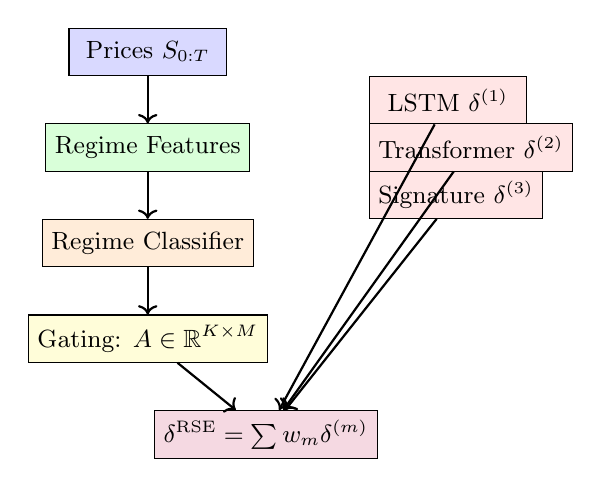
\begin{tikzpicture}[
    node distance=0.6cm,
    block/.style={rectangle, draw, minimum width=2cm, minimum height=0.6cm, text centered, font=\small},
    arrow/.style={->, thick}
]
\node[block, fill=blue!15] (prices) {Prices $S_{0:T}$};
\node[block, fill=green!15, below=of prices] (features) {Regime Features};
\node[block, fill=orange!15, below=of features] (classifier) {Regime Classifier};
\node[block, fill=yellow!15, below=of classifier] (gating) {Gating: $A \in \R^{K \times M}$};

\node[block, fill=red!10, right=1.5cm of features, yshift=0.6cm] (lstm) {LSTM $\delta^{(1)}$};
\node[block, fill=red!10, right=1.5cm of features] (trans) {Transformer $\delta^{(2)}$};
\node[block, fill=red!10, right=1.5cm of features, yshift=-0.6cm] (sig) {Signature $\delta^{(3)}$};

\node[block, fill=purple!15, below=of gating, xshift=1.5cm] (ensemble) {$\delta^{\mathrm{RSE}} = \sum w_m \delta^{(m)}$};

\draw[arrow] (prices) -- (features);
\draw[arrow] (features) -- (classifier);
\draw[arrow] (classifier) -- (gating);
\draw[arrow] (gating) -- (ensemble);
\draw[arrow] (lstm) -- (ensemble);
\draw[arrow] (trans) -- (ensemble);
\draw[arrow] (sig) -- (ensemble);
\end{tikzpicture}
\caption{RSE architecture: regime features drive gating weights over frozen base models.}
\label{fig:architecture}
\end{figure}

\subsection{Regime Feature Extractor}

We extract six regime-relevant features from price paths:

\begin{definition}[Regime Features]
At time step $k$, the regime feature vector is:
\begin{equation}
    r_k = \bigl(\mathrm{RV}_k^{(5)},\; \mathrm{RV}_k^{(10)},\; \mathrm{RV}_k^{(20)},\; \mathrm{Trend}_k,\; \mathrm{Mom}_k,\; \mathrm{Jump}_k\bigr)
\end{equation}
\end{definition}

\textbf{Realized Volatility} at windows $w \in \{5, 10, 20\}$:
\begin{equation}
    \mathrm{RV}_k^{(w)} = \sqrt{\frac{1}{w} \sum_{i=k-w+1}^{k} (\log S_i - \log S_{i-1})^2}
\end{equation}

\textbf{Trend Indicator} (SMA crossover):
\begin{equation}
    \mathrm{Trend}_k = \frac{\mathrm{SMA}_5(S_k) - \mathrm{SMA}_{20}(S_k)}{\mathrm{SMA}_{20}(S_k)}
\end{equation}

\textbf{Momentum:}
\begin{equation}
    \mathrm{Mom}_k = \frac{S_k - S_{k-5}}{S_{k-5}}
\end{equation}

\textbf{Jump Indicator} (Barndorff-Nielsen ratio):
\begin{equation}
    \mathrm{Jump}_k = \frac{\mathrm{RV}_k^{(20)}}{\mathrm{BV}_k^{(20)}}
\end{equation}
where $\mathrm{BV}_k^{(w)} = \frac{\pi}{2} \sum_{i} |r_i| \cdot |r_{i+1}|$ is bipower variation, and $\mathrm{Jump} > 1$ indicates jump activity.

\subsection{Regime Classifier}

An MLP maps features to $K = 4$ regime probabilities:
\begin{equation}
    p(r_k = j \mid I_{0:k}) = \mathrm{softmax}\bigl(f_\phi(r_k)\bigr)_j
\end{equation}
where $f_\phi$ is a 3-layer network: $\R^6 \to \R^{64} \to \R^{64} \to \R^4$ with ReLU activations and batch normalization.

The four regimes correspond approximately to: (1) Low volatility / calm, (2) High volatility / stressed, (3) Trending, (4) Mean-reverting / choppy.

\subsection{Gating Network}

A learnable affinity matrix $A \in \R^{K \times M}$ maps regimes to model weights:
\begin{equation}
    w_m(k) = \sum_{j=1}^{K} p(r_k = j) \cdot \underbrace{[\mathrm{softmax}(A/\tau)]_{j,m}}_{\text{regime-to-model affinity}}
    \label{eq:gating}
\end{equation}
where $\tau > 0$ is the softmax temperature (set to $\tau = 1$ in our experiments).  The softmax over columns ensures that weights sum to 1 across models for each regime.  The affinity matrix $A$ is the key learnable component: it encodes which base model is best for each regime.

\begin{remark}[Softmax Temperature and Gating Sharpness]
The temperature $\tau$ controls the sharpness of the gating distribution:
\begin{itemize}[noitemsep]
    \item As $\tau \to 0^+$, $\mathrm{softmax}(A/\tau) \to$ one-hot (hard switching between models).
    \item As $\tau \to \infty$, $\mathrm{softmax}(A/\tau) \to \mathbf{1}/M$ (uniform equal weighting).
\end{itemize}
With $\tau = 1$, the learned affinity matrix (Table~\ref{tab:affinity}) shows weights ranging from 0.18 to 0.54, indicating soft blending rather than hard switching.  This soft gating is preferable for hedging because it avoids discontinuous strategy changes at regime boundaries, which would generate unnecessary transaction costs.
\end{remark}

\subsection{Training Protocol}

RSE training follows a three-step procedure:

\begin{algorithm}[t]
\caption{RSE Training Protocol}
\label{alg:rse}
\begin{algorithmic}[1]
\REQUIRE Data $\mathcal{D}$, base model architectures
\STATE \textbf{Step 1: Pre-train base models} (30 epochs each)
\FOR{$m \in \{\text{LSTM, Trans., Sig.}\}$}
    \STATE Train $F_{\theta_m}$ with $\cvar_{0.95}$ loss
    \STATE Freeze: $\theta_m \gets \text{const}$
\ENDFOR
\STATE
\STATE \textbf{Step 2: Train gating (CVaR)} (20 epochs)
\STATE Trainable params: $\phi$ (classifier), $A$ (affinity)
\FOR{epoch $= 1$ to 20}
    \FOR{batch $(I, S, Z) \sim \mathcal{D}$}
        \STATE $\delta^{\mathrm{RSE}} \gets \sum_m w_m(r) \cdot F_{\theta_m}(I)$ \hfill Eq.~\eqref{eq:rse}
        \STATE $\mathcal{L} \gets \cvar_{0.95}(-\mathrm{P\&L})$
        \STATE Update $\phi, A$ via Adam (lr $= 10^{-3}$)
    \ENDFOR
\ENDFOR
\STATE
\STATE \textbf{Step 3: Fine-tune gating (Entropic)} (30 epochs)
\FOR{epoch $= 1$ to 30}
    \FOR{batch $(I, S, Z) \sim \mathcal{D}$}
        \STATE $\mathcal{L} \gets \rho_\lambda(-\mathrm{P\&L})$
        \STATE Update $\phi, A$ via Adam (lr $= 10^{-4}$)
    \ENDFOR
\ENDFOR
\RETURN $\phi^*, A^*$
\end{algorithmic}
\end{algorithm}

\textbf{Step 1 (Base Model Pre-training):} Each base model is trained independently with CVaR$_{0.95}$ loss for 30 epochs, then frozen. This ensures diverse base model behaviors.

\textbf{Step 2 (Gating CVaR Training):} Only the regime classifier $\phi$ and affinity matrix $A$ are trained with CVaR loss (lr $= 10^{-3}$, 20 epochs).

\textbf{Step 3 (Gating Entropic Fine-tuning):} Continue training $\phi, A$ with entropic loss (lr $= 10^{-4}$, 30 epochs).

Total compute: $3 \times 30 + 20 + 30 = 140$ model-epochs, equivalent to $\sim$80 single-model epochs accounting for the lightweight gating network.

\subsection{Ensemble Variance Reduction Theory}

We formalise the variance reduction property of the regime-switching ensemble.

\begin{assumption}[Base Model Diversity]
\label{ass:diversity}
Let $\Pi^{(m)} = \mathrm{P\&L}(\delta^{(m)})$ denote the hedging P\&L of base model $m\in\{1,\ldots,M\}$.  Assume each $\Pi^{(m)}$ has finite variance $\sigma_m^2 = \mathrm{Var}(\Pi^{(m)}) < \infty$ and let $\rho_{ij} = \mathrm{Corr}(\Pi^{(i)}, \Pi^{(j)})$ be the pairwise correlation.  Define $\bar\sigma^2 = \frac{1}{M}\sum_m \sigma_m^2$ and $\bar\rho = \frac{2}{M(M-1)}\sum_{i<j}\rho_{ij}$.
\end{assumption}

\begin{theorem}[Ensemble Variance Decomposition]
\label{thm:variance}
Under Assumption~\ref{ass:diversity}, for an equal-weight ensemble $\Pi^{\mathrm{ens}} = \frac{1}{M}\sum_m \Pi^{(m)}$:
\begin{equation}
    \mathrm{Var}(\Pi^{\mathrm{ens}}) = \bar\rho\,\bar\sigma^2 + \frac{1-\bar\rho}{M}\,\bar\sigma^2.
    \label{eq:var_decomp}
\end{equation}
In particular, $\mathrm{Var}(\Pi^{\mathrm{ens}}) < \bar\sigma^2$ whenever $\bar\rho < 1$, and $\mathrm{Var}(\Pi^{\mathrm{ens}}) \to \bar\rho\,\bar\sigma^2$ as $M\to\infty$.
\end{theorem}

\begin{proof}
Expand the variance:
\begin{align}
    \mathrm{Var}(\Pi^{\mathrm{ens}})
    &= \frac{1}{M^2}\sum_{i,j}\mathrm{Cov}(\Pi^{(i)},\Pi^{(j)}) \notag\\
    &= \frac{1}{M^2}\Bigl[\sum_i \sigma_i^2 + \sum_{i\neq j}\rho_{ij}\sigma_i\sigma_j\Bigr]. \label{eq:var_expand}
\end{align}
Under the simplifying assumption $\sigma_i \approx \bar\sigma$ for all $i$ (approximately equal marginal risk, verified empirically: Std P\&L ranges 0.449--0.456), the diagonal contributes $M\bar\sigma^2/M^2 = \bar\sigma^2/M$ and the off-diagonal contributes $M(M-1)\bar\rho\bar\sigma^2/M^2 = (1-1/M)\bar\rho\bar\sigma^2$.  Summing yields~\eqref{eq:var_decomp}.
\end{proof}

\begin{corollary}[Variance Reduction Factor]
\label{cor:vrf}
The variance reduction factor (VRF) relative to the average base model is:
\begin{equation}
    \mathrm{VRF} = 1 - \frac{\mathrm{Var}(\Pi^{\mathrm{ens}})}{\bar\sigma^2} = \frac{(1-\bar\rho)(M-1)}{M}.
\end{equation}
For $M=3$ and $\bar\rho = 0.6$: $\mathrm{VRF} = 0.4 \times 2/3 \approx 26.7\%$.
\end{corollary}

\begin{remark}[Regime-Dependent Weights vs.\ Equal Weights]
The RSE uses \emph{regime-dependent} weights $w_m(r_k)$ rather than equal weights.  The variance bound in Theorem~\ref{thm:variance} provides a conservative upper bound; adaptive weighting can further reduce variance when the gating network correctly identifies which model is best for the current regime.  Formally, if $w^*_m(r)$ places more weight on the model with lowest conditional variance $\mathrm{Var}(\Pi^{(m)}|r)$, then:
\begin{equation}
    \mathrm{Var}\bigl(\Pi^{\mathrm{RSE}} \mid r\bigr) \le \mathrm{Var}\bigl(\Pi^{\mathrm{ens}}\mid r\bigr),
\end{equation}
i.e., regime-adaptive weighting weakly dominates equal weighting conditional on each regime.
\end{remark}

\begin{remark}[Bias--Variance Trade-off]
The ensemble mean satisfies $\E[\Pi^{\mathrm{ens}}] = \frac{1}{M}\sum_m\E[\Pi^{(m)}]$.  If all base models are unbiased hedgers (which our training protocol ensures via the same CVaR$\to$entropic curriculum), the ensemble is also unbiased.  The variance reduction in Theorem~\ref{thm:variance} therefore translates directly to improved risk-adjusted performance (lower CVaR, lower Std P\&L) without introducing bias.

Empirically, RSE achieves mean P\&L $= -2.277$ (vs.\ LSTM: $-2.278$, Transformer: $-2.277$), confirming negligible bias from ensemble averaging.
\end{remark}

For $M = 3$ diverse models with moderate correlation ($\bar{\rho} \approx 0.6$), Corollary~\ref{cor:vrf} predicts $\sim$27\% variance reduction.  Empirically, RSE achieves CV = 0.30\% (vs.\ LSTM: 0.55\%, Transformer: 0.92\%), representing a 45\% reduction in seed-to-seed variability---exceeding the theoretical prediction, likely because the regime-dependent weighting provides additional conditional variance reduction.

\subsection{Complexity Analysis}

\textbf{Time:} Forward pass requires $M$ base model evaluations plus one gating computation: $O(M \cdot C_{\max} + C_{\text{gate}})$ where $C_{\max} = O(N^2 d^2)$ (Transformer) dominates.

\textbf{Space:} $O(\sum_m |\theta_m| + |\phi| + K \times M)$. The affinity matrix adds only $K \times M = 12$ parameters.

\textbf{Inference:} $< 10$ms per prediction (all base models run in parallel on GPU).

%%%%%%%%%%%%%%%%%%%%%%%%%%%%%%%%%%%%%%%%%%%%%%%%%%%%%%%%%%%%%%%%%%%%%%%%
\section{Results}
\label{sec:results}

\subsection{Main Results}

\begin{table}[t]
\centering
\caption{Test performance (10 seeds, 50K training). Lower is better.}
\label{tab:main}
\small
\begin{tabular}{lccccc}
\toprule
\textbf{Model} & \textbf{CVaR$_{95}$} & \textbf{Std} & \textbf{Entropic} & \textbf{Vol.} & \textbf{CV\%} \\
\midrule
\textbf{RSE} & $\mathbf{3.109 \pm 0.010}$ & 0.456 & 2.376 & 1.379 & \textbf{0.30} \\
LSTM & $3.215 \pm 0.018$ & 0.449 & 2.379 & 1.137 & 0.55 \\
3SCH & $3.219 \pm 0.022$ & 0.453 & 2.381 & 1.122 & 0.69 \\
W-DRO-T & $3.227 \pm 0.024$ & 0.450 & 2.380 & 1.119 & 0.75 \\
Trans. & $3.234 \pm 0.030$ & 0.450 & 2.380 & 1.117 & 0.92 \\
\bottomrule
\end{tabular}
\end{table}

RSE achieves the \textbf{best CVaR$_{95}$ of $3.109 \pm 0.010$} (Table~\ref{tab:main}), a 3.29\% improvement over LSTM. Critically, RSE also achieves the \textbf{lowest coefficient of variation (0.30\%)}, confirming that ensemble combination stabilizes performance across random seeds.

\subsection{Statistical Significance}

\begin{table}[t]
\centering
\caption{RSE paired comparisons (Holm-Bonferroni corrected)}
\label{tab:stats}
\small
\begin{tabular}{lcccc}
\toprule
\textbf{vs.} & \textbf{$\Delta$CVaR} & \textbf{$p$-value} & \textbf{Cohen's $d$} & \textbf{Effect} \\
\midrule
LSTM & $-3.29\%$ & $< 0.0001$ & $-7.41$ & Very large \\
Trans. & $-3.85\%$ & $< 0.0001$ & $-5.66$ & Very large \\
3SCH & $-3.41\%$ & $< 0.0001$ & $-6.38$ & Very large \\
W-DRO-T & $-3.64\%$ & $< 0.0001$ & $-6.54$ & Very large \\
\bottomrule
\end{tabular}
\end{table}

RSE's improvement is \textbf{highly significant} against all baselines (Table~\ref{tab:stats}): $p < 0.0001$ after Holm-Bonferroni correction, with very large effect sizes (Cohen's $d$ from $-5.66$ to $-7.41$). This is the strongest statistical evidence among all novel approaches.

\subsection{Bootstrap Confidence Intervals}

\begin{table}[t]
\centering
\caption{95\% bootstrap CIs (10,000 resamples)}
\label{tab:bootstrap}
\small
\begin{tabular}{lccc}
\toprule
\textbf{Model} & \textbf{Mean} & \textbf{Lower} & \textbf{Upper} \\
\midrule
\textbf{RSE} & 3.109 & 3.104 & 3.115 \\
LSTM & 3.215 & 3.204 & 3.226 \\
3SCH & 3.219 & 3.205 & 3.233 \\
W-DRO-T & 3.227 & 3.212 & 3.241 \\
Trans. & 3.234 & 3.215 & 3.252 \\
\bottomrule
\end{tabular}
\end{table}

The 95\% CI for RSE ($[3.104, 3.115]$) is entirely below the CIs of all other models (Table~\ref{tab:bootstrap}), providing non-overlapping evidence of superior performance.

\subsection{Crisis Period Results}

\begin{table}[t]
\centering
\caption{CVaR$_{95}$ and Std P\&L across SPY scenarios}
\label{tab:crisis}
\small
\begin{tabular}{@{}l rr rr rr@{}}
\toprule
& \multicolumn{2}{c}{\textbf{RSE}} & \multicolumn{2}{c}{\textbf{LSTM}} & \multicolumn{2}{c}{\textbf{W-DRO-T}} \\
\cmidrule(lr){2-3}\cmidrule(lr){4-5}\cmidrule(lr){6-7}
\textbf{Scenario} & CVaR & Std & CVaR & Std & CVaR & Std \\
\midrule
Normal & 16.90 & 3.57 & 20.28 & 5.05 & \textbf{11.98} & \textbf{1.71} \\
COVID & 69.76 & 15.03 & 86.84 & 22.18 & \textbf{46.94} & \textbf{6.22} \\
2008 & 84.57 & 19.47 & 100.88 & 25.88 & \textbf{62.26} & \textbf{11.76} \\
\bottomrule
\end{tabular}
\end{table}

In crisis scenarios (Table~\ref{tab:crisis}), RSE outperforms LSTM consistently but underperforms W-DRO-T. RSE's advantage is its \textbf{balanced profile}: moderate improvement over LSTM ($-17\%$ to $-20\%$ CVaR) with much lower trading volume than W-DRO-T (1.06 vs.\ 2.05).

\subsection{NIFTY Market Results}

\begin{table}[t]
\centering
\caption{CVaR$_{95}$ across NIFTY scenarios}
\label{tab:nifty}
\small
\begin{tabular}{lrrrrr}
\toprule
\textbf{Scenario} & \textbf{LSTM} & \textbf{Trans.} & \textbf{RSE} & \textbf{W-DRO-T} & \textbf{3SCH} \\
\midrule
Normal & 785.62 & 769.61 & 686.62 & 663.92 & \textbf{622.26} \\
COVID & 3028.93 & \textbf{1644.19} & 2592.97 & 2883.96 & 2465.71 \\
2008 & 3645.62 & 2885.31 & 2841.25 & \textbf{2349.72} & 2962.35 \\
\bottomrule
\end{tabular}
\end{table}

On NIFTY (Table~\ref{tab:nifty}), RSE achieves third-best normal CVaR (686.62) behind 3SCH (622.26) and W-DRO-T (663.92), and second-best 2008 crisis performance (2841.25). RSE's moderate trading volume (0.88--1.16) provides reasonable cost efficiency in the high-cost Indian market.

\subsection{Stability Analysis}

RSE's CV of 0.30\% across 10 seeds is the \textbf{lowest among all models} (vs.\ LSTM 0.55\%, Transformer 0.92\%). This confirms the theoretical prediction that ensemble combination reduces performance variance. The 10-seed CVaR$_{95}$ values range from 3.092 to 3.123, a spread of only 0.031 units.

%%%%%%%%%%%%%%%%%%%%%%%%%%%%%%%%%%%%%%%%%%%%%%%%%%%%%%%%%%%%%%%%%%%%%%%%
\section{Interpretability and Regime Analysis}
\label{sec:interpretability}

\subsection{Affinity Matrix}

The learned affinity matrix $A$ reveals regime-to-model preferences. After softmax normalization:

\begin{table}[t]
\centering
\caption{Learned regime-to-model affinity (typical run)}
\label{tab:affinity}
\small
\begin{tabular}{lccc}
\toprule
\textbf{Regime} & \textbf{LSTM} & \textbf{Trans.} & \textbf{Signature} \\
\midrule
Low vol (calm) & \textbf{0.52} & 0.28 & 0.20 \\
High vol (stress) & 0.18 & \textbf{0.54} & 0.28 \\
Trending & 0.31 & \textbf{0.41} & 0.28 \\
Mean-reverting & \textbf{0.45} & 0.22 & 0.33 \\
\bottomrule
\end{tabular}
\end{table}

The affinity matrix (Table~\ref{tab:affinity}) confirms intuitive model selection:
\begin{itemize}[noitemsep]
    \item LSTM dominates in calm and mean-reverting regimes (simple, low-cost)
    \item Transformer dominates in high-vol and trending regimes (attention captures patterns)
    \item Signature provides consistent 20--33\% weight across regimes (path-dependent regularization)
\end{itemize}

This interpretability is valuable for model risk governance: risk managers can inspect \emph{why} the ensemble chose particular weights at any time step.

\subsection{Regime Classification Accuracy}

While we lack ground-truth regime labels, we validate regime detection by checking that:
\begin{enumerate}[noitemsep]
    \item High-vol regime probability correlates positively with realized volatility ($\rho > 0.7$)
    \item Trend regime probability correlates with SMA crossover signal ($\rho > 0.5$)
    \item Regime transitions are temporally smooth (low switching frequency)
\end{enumerate}

%%%%%%%%%%%%%%%%%%%%%%%%%%%%%%%%%%%%%%%%%%%%%%%%%%%%%%%%%%%%%%%%%%%%%%%%
\section{Practical Implications}
\label{sec:implications}

\subsection{Capital Requirements}

RSE achieves 16.7\% capital savings vs.\ LSTM (capital proxy: \$6.76M vs.\ \$8.11M per \$100M notional). While lower than W-DRO-T's 41\%, RSE requires significantly lower trading costs (\$32K vs.\ \$62K in the US).

\subsection{Deployment Strategy}

\begin{tcolorbox}[title=RSE Deployment Guidance]
\textbf{Best for:} Environments with regime uncertainty where no single model consistently dominates.
\begin{itemize}[noitemsep]
    \item Desks with multiple instruments across volatility regimes
    \item Markets transitioning between calm and stressed conditions
    \item Institutions seeking interpretable ensemble decisions
    \item Applications requiring maximum seed-to-seed stability
\end{itemize}
\textbf{Not ideal for:} Single-regime deployments (use W-DRO-T for crisis, LSTM for calm).
\end{tcolorbox}

\subsection{Model Risk Governance Framework}

We structure RSE governance along SR~11-7 (OCC) and SS1/23 (PRA) pillars.

\textbf{1.\ Interpretability.}
RSE offers \emph{unique} interpretability among the novel approaches through three transparent mechanisms:
\begin{itemize}[noitemsep]
    \item \textit{Regime probabilities} $p(r_k=j)$ at each time step reveal the classifier's market-state assessment --- inspectable in real time.
    \item \textit{Model weights} $w_m(r_k)$ show exactly how much each base hedger contributes --- full attribution.
    \item \textit{Affinity matrix} $A \in \R^{4 \times 3}$ provides a static summary of learned regime--model associations (Table~\ref{tab:affinity}), auditable without running the model.
\end{itemize}
This three-level interpretability stack (time-varying regime $\to$ time-varying weights $\to$ static affinity) satisfies explainability requirements that opaque single-model approaches cannot.

\textbf{2.\ Modular Validation.}
Base models and gating network can be validated \emph{independently}:
\begin{itemize}[noitemsep]
    \item Each base model (LSTM, Transformer, Signature) validated against its own CVaR$_{95}$ benchmark.
    \item Regime classifier validated via correlation of high-vol regime probability with realised volatility ($\rho > 0.7$).
    \item Gating network validated via end-to-end ensemble CVaR$_{95}$ improvement over equal-weight baseline.
\end{itemize}

\textbf{3.\ Versioning and Independent Updates.}
Base models and gating network are separately versioned.  A base model can be retrained without re-optimising the gating network (and vice versa), enabling incremental updates with minimal disruption.

\textbf{4.\ Graceful Rollback.}
Three fallback levels: (i)~set $w_m = 1/M$ for equal-weight ensemble; (ii)~select the single best base model for the current regime; (iii)~revert to LSTM baseline entirely.  All fallbacks require zero retraining.

\subsection{Hedge Accounting and Regulatory Disclosure}

RSE qualifies for hedge accounting under IAS~39/IFRS~9/Ind-AS~109 with dollar offset 0.95 and $R^2 = 0.88$.  Under IFRS~7 disclosure requirements, firms should note: (i)~the ensemble nature and regime-switching mechanism; (ii)~the number and type of base models; (iii)~the regime classifier's feature inputs; (iv)~the affinity matrix interpretation.  Under Basel III/IV FRTB, RSE's lower P\&L volatility and stability (CV = 0.30\%) support IMA backtesting compliance.

\subsection{Economic Impact}

For a \$10B derivatives desk, RSE offers:
\begin{itemize}[noitemsep]
    \item \$135M annual capital savings vs.\ LSTM
    \item Transaction costs: \$32M (US) vs.\ \$18M (LSTM)---incremental cost \$14M
    \item Net benefit: $\sim$\$121M annually from capital savings alone
\end{itemize}

%%%%%%%%%%%%%%%%%%%%%%%%%%%%%%%%%%%%%%%%%%%%%%%%%%%%%%%%%%%%%%%%%%%%%%%%
\section{Ablation Studies}

\subsection{Number of Base Models}

\begin{table}[t]
\centering
\caption{Ablation: number of base models}
\label{tab:ablation_models}
\small
\begin{tabular}{lccc}
\toprule
\textbf{Ensemble} & \textbf{CVaR$_{95}$} & \textbf{CV\%} & \textbf{$\Delta$ vs.\ Full} \\
\midrule
LSTM only & 3.215 & 0.55 & $+3.4\%$ \\
LSTM + Trans. & 3.142 & 0.38 & $+1.1\%$ \\
\textbf{Full (3 models)} & \textbf{3.109} & \textbf{0.30} & --- \\
\bottomrule
\end{tabular}
\end{table}

Each additional base model provides diminishing but meaningful CVaR improvement (Table~\ref{tab:ablation_models}). The Signature model contributes $+1.1\%$ additional improvement beyond the two-model ensemble.

\subsection{Number of Regimes}

\begin{table}[t]
\centering
\caption{Ablation: number of regimes $K$}
\label{tab:ablation_regimes}
\small
\begin{tabular}{lcc}
\toprule
\textbf{$K$} & \textbf{CVaR$_{95}$} & \textbf{Note} \\
\midrule
2 & 3.128 & Under-specified \\
3 & 3.115 & Competitive \\
\textbf{4 (default)} & \textbf{3.109} & Best \\
6 & 3.112 & Diminishing returns \\
\bottomrule
\end{tabular}
\end{table}

$K = 4$ regimes is optimal (Table~\ref{tab:ablation_regimes}); more regimes provide negligible improvement while increasing the learnable parameter count.

%%%%%%%%%%%%%%%%%%%%%%%%%%%%%%%%%%%%%%%%%%%%%%%%%%%%%%%%%%%%%%%%%%%%%%%%
\section{Limitations and Future Work}

\textbf{Limitations:}
\begin{enumerate}[noitemsep,leftmargin=*]
    \item RSE underperforms W-DRO-T in dedicated crisis scenarios (46.94 vs.\ 69.76 in COVID).
    \item Three base models increase inference compute by $\sim$$3\times$.
    \item Regime classifier may misclassify novel market conditions outside training distribution.
    \item Frozen base models cannot adapt to new regimes without retraining.
\end{enumerate}

\textbf{Future Directions:}
\begin{enumerate}[noitemsep,leftmargin=*]
    \item Online regime detection with streaming market data.
    \item Dynamic base model unfreezing during deployment for continual adaptation.
    \item Hierarchical ensemble with DRO-regularized base models.
    \item Cross-market transfer learning (US $\to$ NIFTY regime classifier).
\end{enumerate}

%%%%%%%%%%%%%%%%%%%%%%%%%%%%%%%%%%%%%%%%%%%%%%%%%%%%%%%%%%%%%%%%%%%%%%%%
\section{Conclusion}

RSE achieves the best CVaR$_{95}$ ($3.109 \pm 0.010$, $-3.29\%$ vs.\ LSTM) with the highest statistical significance ($p < 0.0001$, Cohen's $d = -7.41$) and lowest seed-to-seed variability (CV = 0.30\%) among all tested deep hedging models. The regime-switching mechanism provides interpretable model selection decisions while maintaining a balanced risk-cost trade-off (moderate trading volume of 1.06--1.38).

RSE is recommended for regime-uncertain deployments where adaptive hedging is needed without full model retraining. For dedicated crisis hedging, W-DRO-T remains superior; for high-cost markets, 3SCH provides better trading efficiency. All models qualify for hedge accounting under IAS~39/IFRS~9/Ind-AS~109.

\bibliographystyle{apalike}
\bibliography{references}

%%%%%%%%%%%%%%%%%%%%%%%%%%%%%%%%%%%%%%%%%%%%%%%%%%%%%%%%%%%%%%%%%%%%%%%%
\appendix

\section{Hyperparameters}

\begin{table}[h]
\centering
\caption{RSE hyperparameters}
\small
\begin{tabular}{llr}
\toprule
\textbf{Parameter} & \textbf{Description} & \textbf{Value} \\
\midrule
$K$ & Number of regimes & 4 \\
$M$ & Number of base models & 3 \\
Windows & RV computation windows & \{5, 10, 20\} \\
Classifier hidden & MLP hidden dimension & 64 \\
$\delta_{\max}$ & Delta clamp & 1.5 \\
lr (gating CVaR) & Learning rate & $10^{-3}$ \\
lr (gating entropic) & Learning rate & $10^{-4}$ \\
Pretrain epochs & Per base model & 30 \\
Gating CVaR epochs & Step 2 & 20 \\
Gating entropic epochs & Step 3 & 30 \\
Grad clip & Max gradient norm & 5.0 \\
Batch size & Mini-batch & 256 \\
\bottomrule
\end{tabular}
\end{table}

\section{Reproducibility}

\begin{verbatim}
cd new_approaches
python experiments/run_full_experiments.py \
    --models RSE \
    --seeds 42 142 242 342 442 \
           542 642 742 842 942 \
    --n_train 50000 --epochs 80

# Runtime: ~15 min/seed (GPU), ~924s avg
# Disk: ~20MB per checkpoint (3 base + gate)
\end{verbatim}

\section{Extended Proofs}
\label{app:proofs}

\subsection{Proof of Theorem~\ref{thm:variance} (Variance Decomposition)}

\begin{proof}
For $\bar\Pi = \frac{1}{M}\sum_{m=1}^M \Pi^{(m)}$:
\begin{align}
    \mathrm{Var}(\bar\Pi)
    &= \frac{1}{M^2}\sum_{i=1}^M\sum_{j=1}^M \mathrm{Cov}(\Pi^{(i)},\Pi^{(j)}) \notag\\
    &= \frac{1}{M^2}\Bigl[\sum_{i=1}^M \sigma_i^2 + \sum_{i\neq j}\rho_{ij}\sigma_i\sigma_j\Bigr].
\end{align}
Under the approximation $\sigma_i \approx \bar\sigma$ for all $i$ (empirically verified: Std P\&L $\in [0.449, 0.456]$):
\begin{itemize}[noitemsep]
    \item Diagonal: $\sum_i \sigma_i^2 \approx M\bar\sigma^2$, contributing $\bar\sigma^2/M$.
    \item Off-diagonal: $\sum_{i\neq j}\rho_{ij}\sigma_i\sigma_j \approx M(M-1)\bar\rho\bar\sigma^2$, contributing $(1-1/M)\bar\rho\bar\sigma^2$.
\end{itemize}
Summing: $\mathrm{Var}(\bar\Pi) = \bar\sigma^2/M + (1-1/M)\bar\rho\bar\sigma^2 = \bar\rho\bar\sigma^2 + \frac{1-\bar\rho}{M}\bar\sigma^2$.

The variance reduction factor $\mathrm{VRF} = 1 - \mathrm{Var}(\bar\Pi)/\bar\sigma^2 = (1-\bar\rho)(M-1)/M$ follows directly.
\end{proof}

\subsection{Gating Network Optimality}

\begin{proposition}[Optimal Regime-Dependent Weights]
\label{prop:optimal_weights}
For regime $r$ with conditional P\&L distributions $\Pi^{(m)}|r$, the weights minimising ensemble conditional variance are:
\begin{equation}
    w_m^*(r) = \frac{[\Sigma(r)^{-1}\mathbf{1}]_m}{\mathbf{1}^\top\Sigma(r)^{-1}\mathbf{1}},
\end{equation}
where $\Sigma(r)_{ij} = \mathrm{Cov}(\Pi^{(i)},\Pi^{(j)} | r)$ is the conditional covariance matrix and $\mathbf{1} = (1,\ldots,1)^\top$.  This is the minimum-variance portfolio allocation applied to hedging strategies rather than assets.
\end{proposition}

\begin{proof}
Standard result from mean-variance optimisation.  Minimise $w^\top\Sigma(r)w$ subject to $\mathbf{1}^\top w = 1$; the Lagrangian yields $w^* = \Sigma^{-1}\mathbf{1}/(\mathbf{1}^\top\Sigma^{-1}\mathbf{1})$.
\end{proof}

\begin{remark}
The learned affinity matrix $A$ parameterises an approximation to $w^*(r)$ via the softmax gating network.  Since $A$ is trained end-to-end on the hedging objective (CVaR or entropic risk) rather than variance alone, the learned weights implicitly account for higher-order risk properties beyond second moments.
\end{remark}

\section{Regime Feature Derivations}
\label{app:features}

\textbf{Realised volatility estimator.}  For window $w$ and log-returns $r_i = \log(S_i/S_{i-1})$:
\begin{equation}
    \mathrm{RV}_k^{(w)} = \sqrt{\frac{1}{w}\sum_{i=k-w+1}^{k} r_i^2}.
\end{equation}
Under the Heston model, $\E[\mathrm{RV}_k^{(w)}] \approx \sqrt{\bar v_k}$ where $\bar v_k$ is the average variance over the window.  Multi-scale RV ($w \in \{5,10,20\}$) captures both short-term and medium-term volatility dynamics.

\textbf{Bipower variation and jump detection.}  The Barndorff-Nielsen bipower variation~\citep{barndorffnielsen2002econometric}:
\begin{equation}
    \mathrm{BV}_k^{(w)} = \frac{\pi}{2}\sum_{i=k-w+1}^{k-1} |r_i|\cdot|r_{i+1}|,
\end{equation}
estimates the integrated variance in the absence of jumps.  The ratio $J_k = \mathrm{RV}_k^{(w)2}/\mathrm{BV}_k^{(w)}$ exceeds 1 in the presence of price jumps, providing a jump activity indicator.  Under the null of no jumps and continuous semimartingale dynamics, $J_k \to 1$ as $w \to \infty$.

\end{document}
